\documentclass[12pt]{article}
\usepackage[utf8]{inputenc}
\usepackage[T1]{fontenc}
\usepackage{titlesec}
\usepackage[inline]{enumitem}
\usepackage[left=2.54cm,top=3cm,right=2.54cm,bottom=3cm]{geometry}
\usepackage[sorting=none, style=numeric-comp]{biblatex}
\usepackage{hyperref}
\usepackage{graphicx}
% \usepackage{upgreek}
\usepackage{setspace}
% \usepackage{longtable}
\usepackage{tabularx}
\usepackage{framed}
% \usepackage{eurosym}
\usepackage{listings}
\usepackage{rotating}
\usepackage[table]{xcolor}
\usepackage[acronym,toc,nogroupskip,nopostdot]{glossaries}
\usepackage{glossary-mcols}


% \graphicspath{ {00images/} }
\DeclareGraphicsExtensions{.png,.pdf,.jpg}
% \DeclareGraphicsExtensions{.pdf,.png} % - CHANGE TO THIS

\addbibresource{mendeley.bib}
\setlength{\parindent}{1cm}

% Acronyms %%%%%%%%
\makeglossaries

\newacronym{iot}{IoT}{Internet of things}
\newacronym{gps}{GPS}{Global Positioning System}
\newacronym{gsm}{GSM}{Global System for Mobile Communication}
\newacronym{osi}{OSI}{Open Systems Interconnection}
\newacronym{mac}{MAC}{Medium Access Control}
\newacronym{llc}{LLC}{Logical Link Control}
\newacronym{udp}{UDP}{User Datagram Protocol}
\newacronym{tcp}{TCP}{Transmission Control Protocol}
\newacronym{wsn}{WSN}{Wireless sensor network}
\newacronym{pdu}{PDU}{Protocol Data Unit}
\newacronym{smacs}{SMACS}{Self-Organizing Medium Access Control for Sensornets}
\newacronym{leach}{LEACH}{Low-energy adaptive clustering hierarchy}
\newacronym{tdma}{TDMA}{Time-division multiple access}
\newacronym{cdma}{CDMA}{Code-division multiple access}
\newacronym{fdma}{FDMA}{Frequency-division multiple access}
\newacronym{spin}{SPIN}{Sensor Protocols for Information via Negotiation}
\newacronym{pegasus}{PEGASIS}{Power-Efficient Gathering in Sensor Information Systems}
\newacronym{rmst}{RMST}{Reliable Multisegment Transport}
\newacronym{esrt}{ESRT}{Event-to-Sink Reliable Transport}
\newacronym{coda}{CODA}{Congestion Detection and Avoidance}
\newacronym{pan}{PAN}{Personal Area Network}
\newacronym{aes}{AES}{Advanced Encryption Standard}
% \newacronym{}{}{}
% \newacronym{}{}{}
% \newacronym{}{}{}
% \newacronym{}{}{}

\makeglossaries

%%%%%%%%%%%%%%%%%%% 

\begin{document}
% 
\tableofcontents
% \pagebreak

% \begin{singlespacing}
\setglossarystyle{mcolindex}
\printglossary[type=\acronymtype, title=List of acronyms and abbreviations, toctitle=List of acronyms and abbreviations, nonumberlist]
\printglossary
% \end{singlespacing}

\pagebreak

\section{Introduction}
% 
In today’s world of outsourcing production to other country than the one where the development was done in, is a common practice. Reasons varies, but mostly, it is the economical aspect. This however, raises many problems within logistics, meaning getting products from the plant on one side of the globe to a warehouses and customers on the other. Keeping track of every container leaving the plant on truck’s trailer to a port, to be loaded on a huge cargo ship with hundreds of others and subsequently being unloaded at the destination port to the right truck’s trailer and getting it to a given warehouse, poses a challenge. What is even more, as a wide range of products are being transported, each product requires a different kind of handling in means of temperature in a container, fragility of products or speed of shipment. But how to collect all of these data and provide enhanced supply chain management?
One of ways to go is the use of \acrshort{iot}\footnotemark. ``\textit{The \acrfull{iot} is a system of interrelated computing devices, mechanical and digital machines, objects, animals or people that are provided with unique identifiers and the ability to transfer data over a network without requiring human-to-human or human-to-computer interaction}'' \cite{MargaretRouse2016WhatWhatIs.com}. In the given problem in logistics, each object – container, is able to provide loads of useful data which may be collected. Collection of such data may be done with help of various sensors which may be deployed in each container. By interconnecting them, each container will have its own small network, made of several slave sensors and a master device. In this use case, the focus will be put into the use of such networks on cargo ships to provide a crew with information from each container in a central system, as well as providing a shipment client with details about his container.
% 
\footnotetext{\url{http://www.businessinsider.com/internet-of-things-logistics-supply-chain-management-2016-10?r=US&IR=T&IR=T}, accessed 05-05-2018}

To address this problem, the suggested solution is to equip each container with a hub and a set of sensors which may be added on demand, interconnecting the hub with a central receiver and providing information to a central system. In this project, the main area of research will be analysis of different wireless standards which may fit the solution as well as design of architecture of such a system.

Lets take John as an example. John is the owner of a shop chain based in Denmark, selling party decorations, costumes and gadgets. It is also a country, where their own designs are. However, as it is cheaper for them to have a production in a country with cheap work force, they are produced in China, from where all other stuff are bought as well. John would like to keep track of all containers shipped from China to Denmark, as well as being updated about conditions within container. Therefore, he decides that all of them should be equipped with \acrshort{gps}, temperature monitor, motion sensor and of course a \acrshort{gsm} module with hub. Because of that, he can track where a container is live, check whether the requested temperature for transportation is met, see when a container is being opened and have access to this information anytime and anywhere in the world. This a good solution for when a container is on land. However, when it is loaded on a cargo ship, sailing on the ocean, there is no signal from base station and therefore communication with satellite would be needed which is relatively expensive\footnotemark.
% 
\footnotetext{\url{https://www.quora.com/Why-is-satellite-Internet-service-so-relatively-expensive-and-not-available-worldwide}, accessed 05-05-2018}

One of many solutions to this problem, would be having a cargo ship equipped with several hubs to which containers on board would be periodically pushing information and these will be collected in the central system. This information then, would be every few minutes sent via satellite to central server and accessible for a client. Because of that, the cost for internet connection on board would be lower as there would be only one from the central system instead of many from each container, and crew would have precise information about each container, knowing if there was some problem.
\section{Architecture}

The main actors in the system are clear: the heart of the problem is the temperature-sensitive cargo that needs to be transported. This cargo is loaded in the refrigerated containers, also known as reefers. Each type of cargo requires different temperature and air composition, so these settings differ among the reefers. There is at least one temperature sensor and one gas monitoring sensor in every reefer. Reefers, together with regular containers and other cargo are loaded onto a vessel and transported across the sea.

When the temperature and the air quality are monitored, the goal is to transfer the data to:

\begin{itemize}
    \item \textit{Collection point/database}, so that the transport company can prove to its customers that the cargo maintained the desired temperature throughout the whole duration of the journey. Some systems allow the customer to monitor the data from the container in real time.
    \item \textit{Ship bridge}, to ensure that the temperature in the container is not too high (i.e. due to a power loss) and that the systems are operating normally (i.e. there is no fire in the container). 
\end{itemize}

The simplest architecture for this transfer of data from every container would probably consist of sensors submitting data directly to the collection point. It is obvious that this probably has many drawbacks. Even if there are only two sensors in each containers, there are still hundreds of containers on a ship. If there was only one collection point for all of Maersk’s fleet, this point would need to handle connections from tens of thousands devices, since there are hundreds of ships in operation worldwide.

//THIS IS SHOWN IN FIGURE

A solution to this problem is to introduce a \textit{hub}. Hub is a cluster node, that collects, processes and re-transmits data to the sink, but it does not sense any data by itself. The sensors in the container would connect to a hub and the hub would then connect to sink. This reduces the number of connections that need to be handled by the sink and also limits the necessary transmission power of the sensor. The problem then lies in the relative position of the hub. If the hub is positioned too close to the sensors, we can lower the necessary transmission power of the sensors, but more hubs per vessel would be needed to cover all of the containers. If the hub is too far from the sensors, less hubs per vessel would be needed, but the range of the sensors would need to increase. The lesser the hubs are there, the fewer communication links to the sink are needed. In a shipping scenario, where vessels are often out of reach of the traditional \acrshort{gsm} band and satellite communication must be used to transmit data to shore. Satellite link is a scarce resource and limiting the amount of satellite connections required is beneficial.

//SHOWN IN A FIGURE TOO, I GUESS

An alternative solution to compromise between the sensor transmit power and number of hubs required, is to introduce a second-level hub. Second-level hubs are the middle man between first-level hubs and the sink. Sensors connect and transfer their data to the first-level hub. This hub processes the data and forwards it to the second-level hub. Second-level hub collects the data and forwards them to the sink in batches. A plausible placements of the hubs could be inside a container for the first-level hub and on the bridge for the second-level hub. In this setup, the sensors only need to transmit their data over a short distance, therefore the power consumption can be reduced. The second-level hub collects data from the whole vessel before forwarding them to the sink. If there only is one second-level hub per vessel, the number of satellite links required is reduced.
%
% 
% \footnotetext{This does not neccessarily refer to the physical distance to the sensors, rather than relative position in the architecture with respect to}

% 
\section{Overview of WSN layers}  \label{sec:layers}

To analyse various existing protocols, we must first learn about how a \acrlong{wsn} is built. Research suggests that while some parameters are the same as in other networks, such as Internet, other parameters are significantly different~\cite{Sohrabi2000ProtocolsNetwork}. The main limitation of the \acrshort{wsn} lies in the fact that the sensors are often battery powered and thus need to be conscious with their energy expenditure. Another implication of this is, that sensors often do not have enough computational power to calculate advanced cryptographic algorithms.

In the following section we will investigate the physical, MAC, network and transport layers, from the perspective of a WSN.
\subsection{Physical layer}
Physical layer is the first layer of the OSI reference model. The main role of the physical layer is the transmission of electrical, optical or radio signal over transmission medium. This layer describes the transmission medium itself (whether it is metallic or optical cable, wireless, etc.) and its properties, network interface parameters and nature of transmitted signal; in other words, the physical properties and characteristics of the transmitted signal and the transfer medium. The physical layer does not understand the transmitted data itself, it only sees it as a stream of bits and is responsible for their transmission. It provides service to the Data link layer.

Main functions and services offered by this layer are:
\begin{itemize}[noitemsep]
    \item Establishing and termination of connection with communication medium
    \item Effective sharing of resources between multiple users (e.g. conflict resolution) or is this Data link?
    \item Modulation or conversion of digital data from the user’s device to the corresponding signals transmitted by the communication channel 
    \item Traffic management
    \item Physical topology
    \item Transmission mode and rate
    \item Physical characteristics
    \item Bit representation
\end{itemize}

Components of physical layer may be divided into passive and active components. Active components are those that amplify or modify a transmitted signal. The most common devices are transceivers, hubs or repeaters. Passive components, unlike active ones, do only transmit a signal and do not modify, amplify or create it in any way, for example cables or connectors.

In case of IoT and \acrfull{wsn}, data are transmitted wirelessly and wireless networks as well as their physical layer has different characteristics to wired ones. To be able to send any kind of information or data over the air, there must be a certain portion of the radio spectrum must be allocated for this purpose. As it may be seen in~\ref{fig:freq-alloc}, the radio spectrum is already very crowded and so this resource is very sacred. Most of the spectrum’s frequency bands are already given their use for different purposes like TV signal transmission, FM radio or maritime communication. Therefore, if a new technology emerges and would like to use a frequency band of the spectrum, it can either pay and get a licensed band or can use special license-free bands like ISM radio band (industrial, scientific and medical) or U-NII band, which may be used freely. That is what most physical layer protocols does, make use of a freely available bands, which makes a technology cheaper, but the interference is higher as the band is more crowded.

\begin{figure}[ht]
    \centering
    
    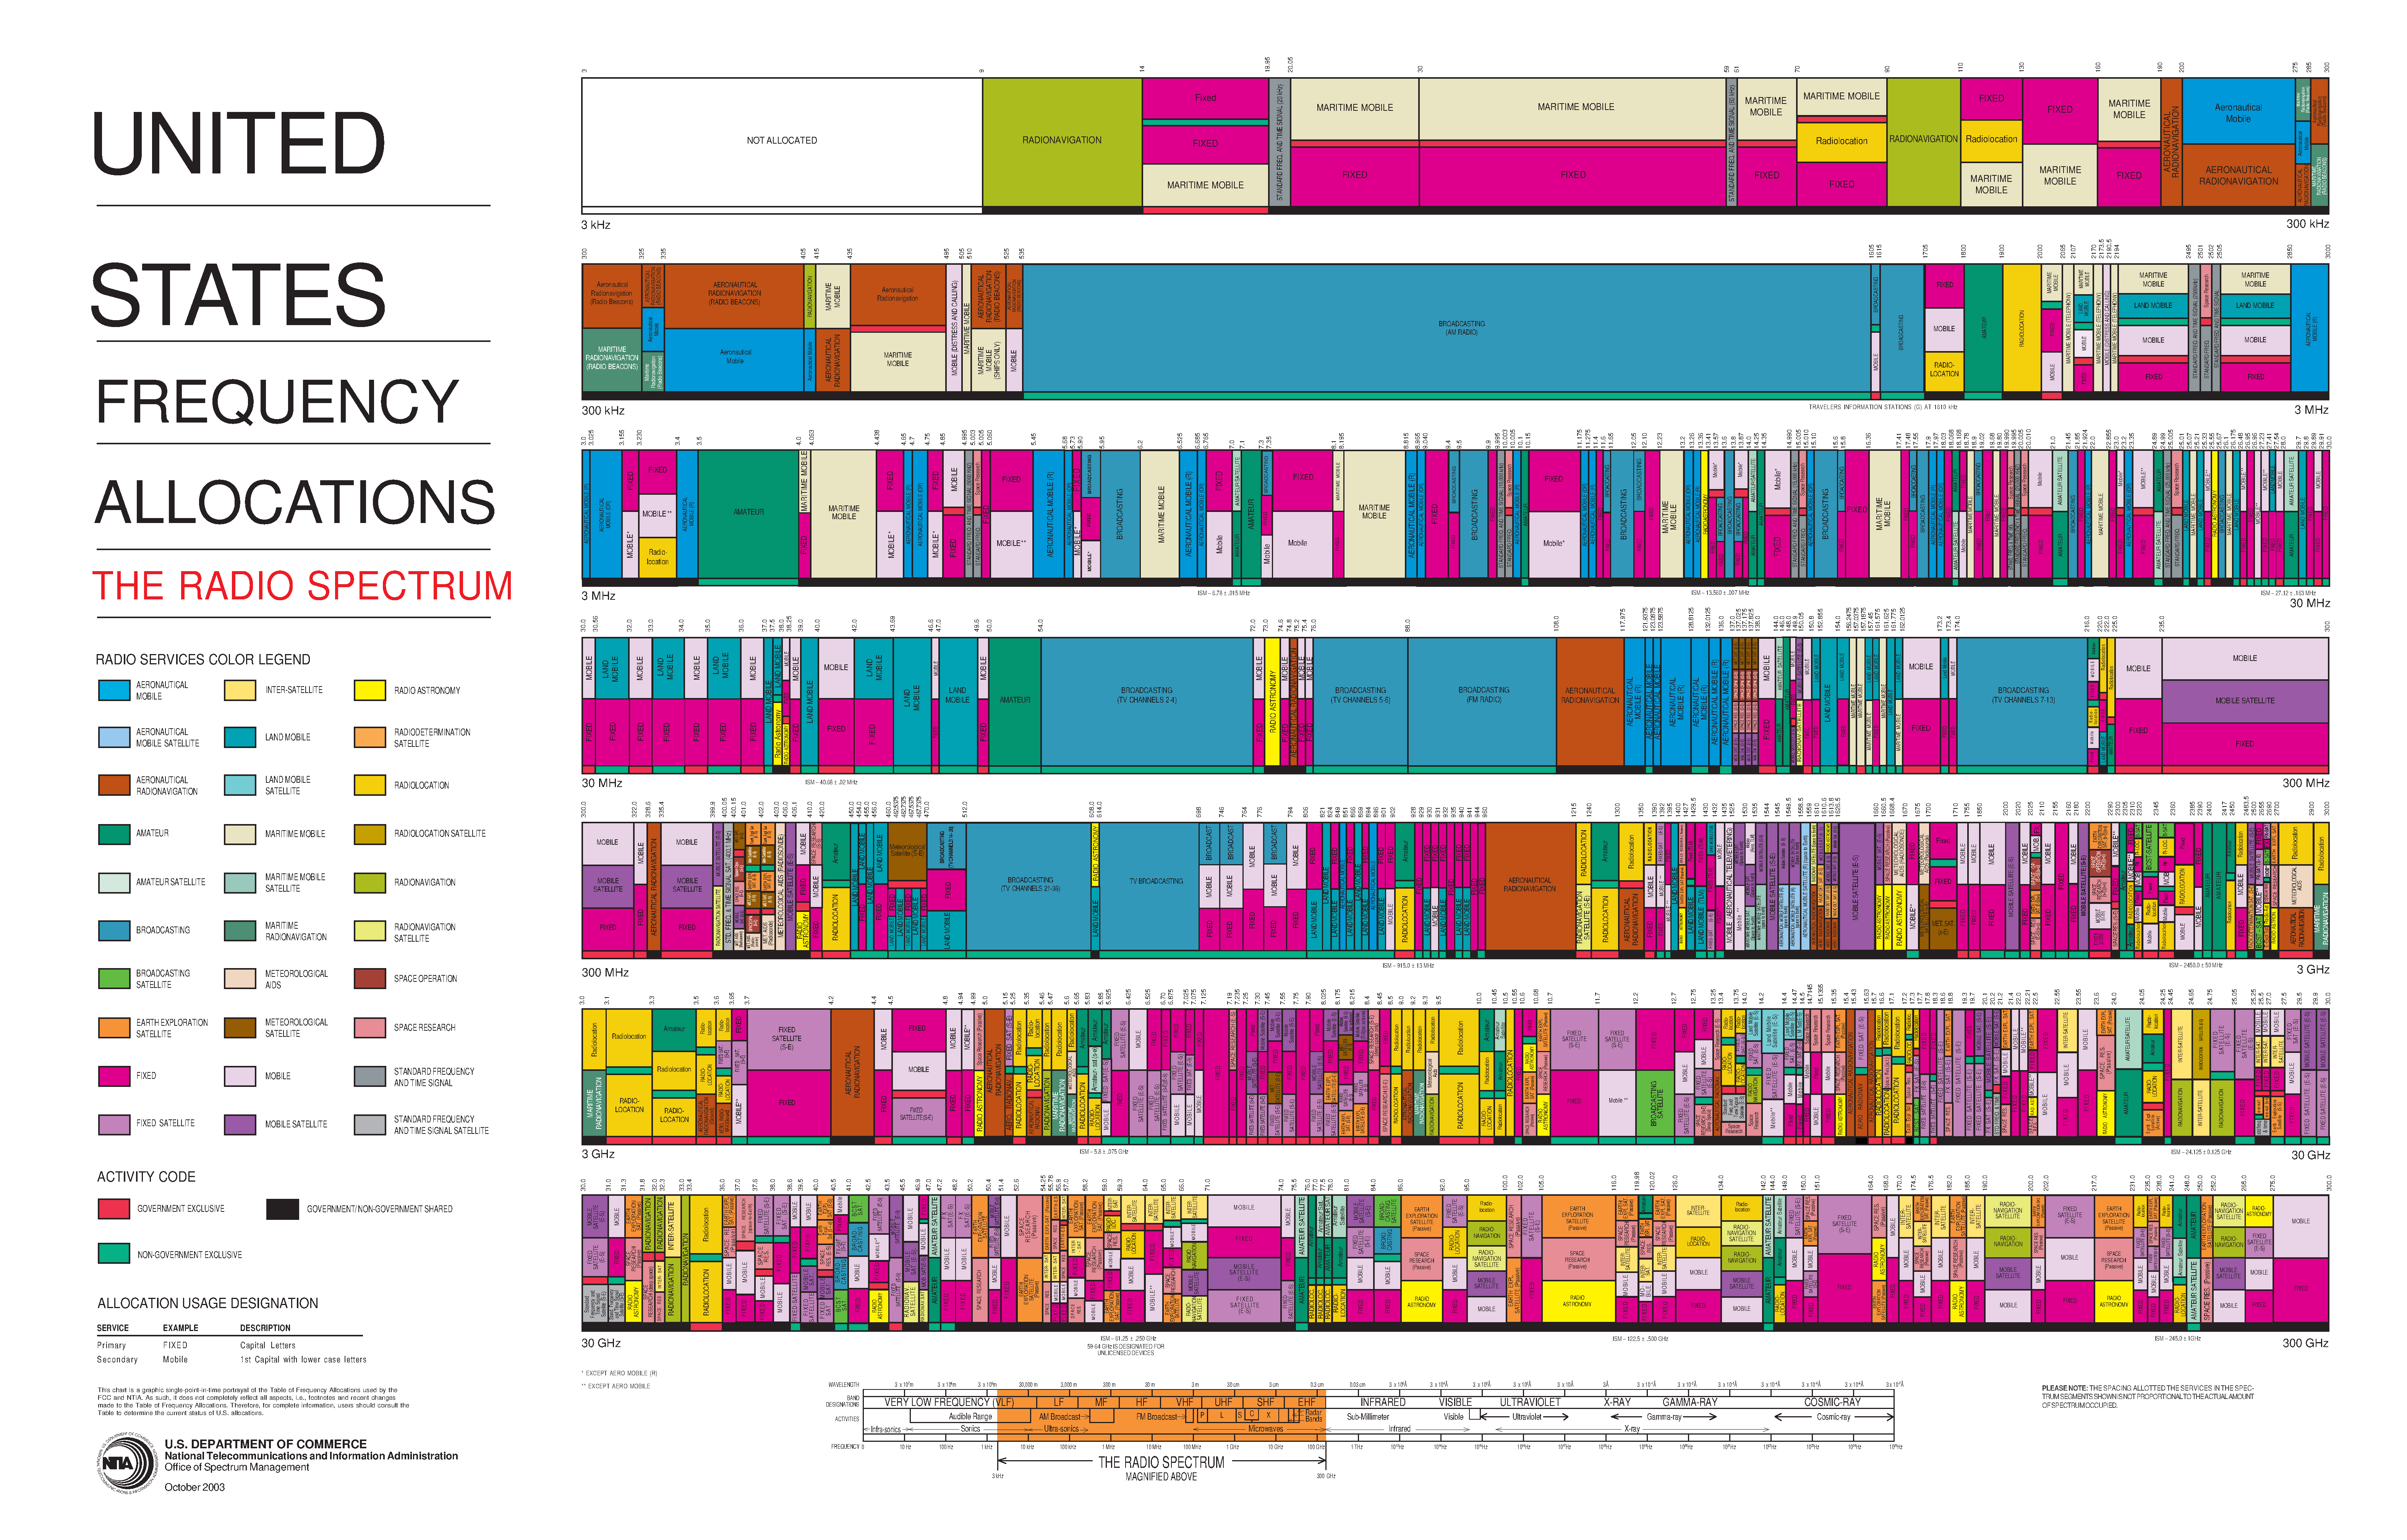
\includegraphics[width=\textwidth]{00images/freq-alloc}
    \caption{Frequency allocations of the spectrum. Source: \url{https://www.ntia.doc.gov/files/ntia/publications/2003-allochrt.pdf}, accessed 11-05-2018}
    \label{fig:freq-alloc}
\end{figure}

Spectral efficiency says how much of an information can be send over a given portion of frequency spectrum, how well the frequency spectrum is utilised. This is important in wireless networks, as frequency bands are limited and the higher the utilisation the better. Another important aspect of wireless transmission is the range. Unlike the wired communication where cables used may be very long, interference low and bandwidth high as dedicated cables are used, wireless communication suffers from these much more as the signal wave travels through the air and is interfered with other signals and propagation loss. As it may be seen in~\ref{fig:radio-spectrum}, choosing the right frequency band is crucial, because the lower frequencies have higher range, devices are cheaper to produce, but bandwidth is smaller while the higher the frequency band, the higher the bandwidth but smaller the range. On top of that, in \acrshort{iot} devices are many times battery powered, meaning they must be power efficient and a ration between signal strength, power consumption and bandwidth must be chosen carefully.

\begin{figure}
    \centering
    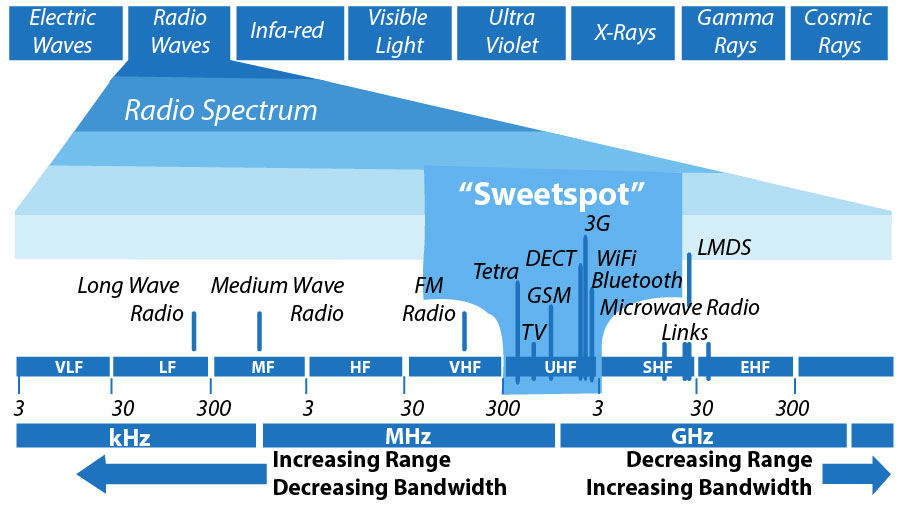
\includegraphics[width=0.8\textwidth]{00images/radio-spectrum-3}
    \caption{Radio spectrum division. Source: \url{https://nuzeal.com/index.php/radio-spectrum-availability/}, accessed 11-05-2018}
    \label{fig:radio-spectrum}
\end{figure}{}

There are several metrics that can be used to assess the performance of a physical layer. These metrics are listed in Table~\ref{tab:metrics-physical}.

\begin{table}[ht]
     \centering
    \begin{tabularx}{\textwidth}{|l|X|p{5em}|}
    \hline
    \textbf{Metrics}&\textbf{Description}&\textbf{Relevance}\\
    \hline
    Range&Range is a metrics that tells how far from transmitter may a message be successfully received by a receiver.&••\\
    Throughput&Throughput is the rate of successful message delivery through the communication channel.&•\\
    Spectral efficiency&Spectral efficiency tells how much the frequency band is utilised.&•\\
    Power consumption&Power consumption describes how much power is need by a device to send a message of the same size.&••\\
    \hline
    \end{tabularx}
    
    \caption{Metrics used to evaluate protocols in physical layer.}
    \label{tab:metrics-physical}
\end{table}{}

\subsection{Data link layer}
Data link layer is the second layer of the \acrshort{osi} reference model. It consists of \acrfull{mac} and \acrfull{llc} layer. The \acrshort{mac} layer is responsible for regulating the access to the shared communication medium among nodes, while the \acrshort{llc} layer is used to define and control properties of the \acrshort{mac} layer, to shield the upper layers of the model from the physical network and provide inter-operability  across different types of networks. Since the use of \acrshort{llc} layer in practice is limited~\cite{Sohraby2007WirelessApplications}, we will further focus on the \acrshort{mac} layer.

The medium access control layer is responsible for managing the access to the shared communication medium. In wireless networks, it is usually the case that only one device can use the wireless medium at a time, otherwise the interference of wireless signals will render the transmission invalid. The \acrshort{mac} layer resolves this problem, by maintaining a scheme on how and when each node can transmit. The design of the \acrshort{mac} layer is the ``\textit{major determining factor in Wireless Sensor Network performance}''\cite{Sohraby2007WirelessApplications}. 

However, there are several complexities associated with designing this layer. Besides the overall complexity spanning through the whole system, such as limited performance of the devices due to size and power constraints, \acrshort{mac} layer must also account for eventual movement of the devices. Furthermore, when the \acrshort{mac} layer needs to coordinate access to a medium, often the same medium must also be used for this coordination effort. This coordination effort results in better decisions of nodes when to transmit and when not to. The better the decisions, the fewer collisions appear and the less wasted time and transmission power. However, this coordination effort imposes overhead on the communication channel -- on top of the actual data from the sensors, some sort of coordination needs to be added. As~\cite{Sohraby2007WirelessApplications} notes, a trade-off between the quality of the decision and the amount of overhead incurred needs to be made.

There are several metrics that can be used to asses the performance of a \acrshort{mac} layer. 

\begin{table}[ht]
    \centering
    \begin{tabularx}{\textwidth}{|l|X|p{5em}|}
    \hline
    \textbf{Metrics}&\textbf{Description}&\textbf{Relevance}\\
    \hline
    Delay&Sohraby et. al. defines delay as the amount of time packet spends in the MAC layer before it is transmitted successfully~\cite{Sohraby2007WirelessApplications}.&•\\
    \hline
    Throughput&Throughput is the rate of successful message delivery through the communication channel.&•\\
    \hline
    Scalability&Scalability is the ability of the protocol to maintain its usual performance with increasing amount of devices&•••\\
    \hline
    Stability&Stability is a metrics that measures how well can the system resist changes of the traffic load over a period of time.&•••\\
    \hline
    Fairness&Fairness of a MAC protocol describes how well does the protocol distribute resources among the devices without significantly limiting the throughput.&••\\
    \hline
    \end{tabularx}
    \caption{Comparison of different MAC layer metrics. The \textit{Relevance} column is an approximation of how relevant this metric is in the reefer shipping scenario.}
    \label{tab:mac-metrics}
\end{table}

Generally, the MAC protocols can be divided into two groups: contention-free and contention-based protocols. Contention-free protocols only allow one device to access the medium at the time. This group can be further divided into \textit{fixed assignment} and \textit{dynamic assignment}, depending on how the protocol assigns communication slots to devices. Contention-based protocols allow multiple devices to access the medium at the same time, but provide a recovery mechanism, shall a collision occur. Figure~\ref{fig:mac-categories} displays this grouping.

\begin{figure}[ht]
    \centering
    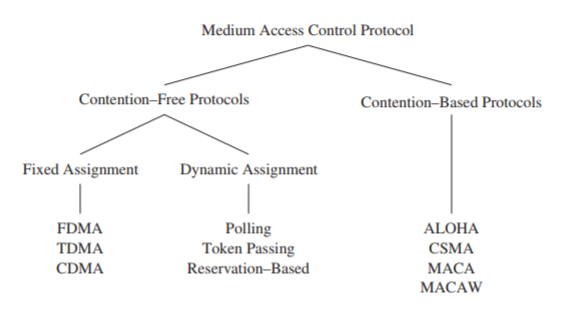
\includegraphics[width=0.8\textwidth]{00images/mac-categories}
    \caption{Categorisation of MAC protocols, according to channel access. Few examples are given for each category. Taken from~\cite{2011MediumControl}.}
    \label{fig:mac-categories}
\end{figure}
\subsection{Network layer}
The network layer is the third layer of the \acrshort{osi} reference model. It enables interconnection of multiple networks into larger ones, and provides means for a clear and logical identification of a computer on any network. This layer provides functional and procedural means of transmitting variable-length data sequences from source to target by one or more networks, while being in charge of the quality of service required by the transport service. 

On this layer, a header is added which encapsulates the \acrfull{pdu} coming from transport layer which is a segment. The header specifies information needed for successful transmission, such as logical addresses. After adding this header, the \acrshort{pdu} is called a packet.

From a network layer perspective, the entire ``global'' network environment is partitioned into networks and subnets. Every network (subnet) has its own address that uniquely identifies it, and each computer has its own unique address in each of these networks. By having the network address and the computer address, it is possible to uniquely identify the computer on any network. This address belongs to logical addresses because it depends on where your computer is located. If we transfer a computer from one network to another, its network (logical - IP) address will change, while its physical address -- the \acrshort{mac} address -- remains the same.

Network layer tasks include:
\begin{itemize}[noitemsep]
    \item Unambiguous addressing
    \item Identifying the optimal data delivery path between the sender and the recipient
    \item Packet creation
    \item Transferring packets to the end recipient
    \item Re-composition of packets at the recipient
\end{itemize}

When a sender sends a packet to a recipient, it may send it via its predefined router for delivery. The router from the packet reads the address of the recipient, scans its subnet database, finds out to which of them the packet belongs to, and through which next nearest router the packet has to go. Once this information is obtained, it sends the packet to the specified router. This process is repeated until the packet has reached the destination network.

When sending a packet through wireless sensor network, it is often viable to use multi-hop approach; reason is that a node sending data to the base station may be far away, which means it would need to use much more energy for transmission compared to as if it was close. On top of that if there are many nodes and each of them is directly connected to a base station, a lot of interference is created when accessing the channel. Therefore, nodes must participate and forward data towards a sink; data are send to a nearest node, which forwards it further until destination is reached as it may be seen in Figure~\ref{fig:multihop}.

As already mentioned, a sender may send a packet to a predefined router and use a predefined path for delivery. However, there is a problem with selecting the best routing path, and its solution is one of the main network layer tasks. This problem is complicated by the fact that the shortest route is not always the best. The reason for the shortest path not always being the best is that there might be congestion on a path, some link may be unreliable, or it may be too power consuming to send a packet via the path. Frequently the route selection criterion is the time by which a packet can be delivered via a route; some routing algorithms determines a path by congestion between routers, while others make decisions based on average performance over a long period of time. Transfer reliability may be used as a criterion as well. Therefore, a routing algorithm should be carefully designed to meet traffic requirements and extend lifetime of the network as much as possible, because nodes may be battery powered.

\begin{figure}
    \centering
    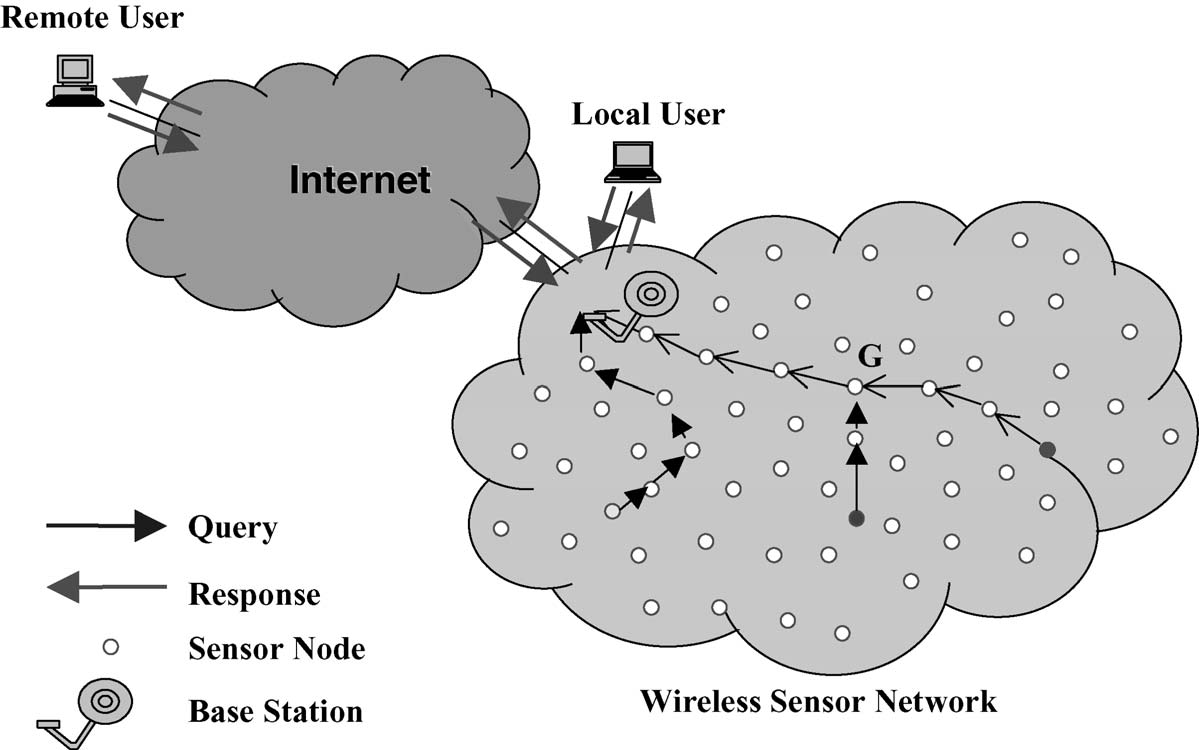
\includegraphics[width=0.8\textwidth]{00images/multihop}
    \caption{Multi-hop node communication. Taken from~\cite{Sohraby2007WirelessApplications}.}
    \label{fig:multihop}
\end{figure}

Several strategies for routing algorithms exists: proactive, reactive and hybrid strategies. Proactive strategy is based on routing tables which needs to be updated and contain global information about nodes across the network, based on them the optimal route is calculated beforehand. Such strategy is not vital in huge \acrshort{wsn}. The reactive strategy on the other hand, discovers the best path on demand, without prior knowledge of nodes information across the network. The last strategy, the hybrid one is a mix of proactive and reactive strategies, where nodes are organised in clusters. Communication within cluster use proactive strategy while in between cluster the reactive one is used.

In \acrshort{wsn} networks there are several routing techniques/classes being used to achieve requirements fulfilment set by customer, e.g. power limitation, maximum delay and packet loss or resource limitation. A first class has a flat network approach, meaning all nodes are considered to be on the same level – peers. Advantages of such architecture are possible detection of multiple paths and minimal overhead and low cost. Next class has a hierarchical network approach, where nodes are organised into clusters with the presence of a cluster master which serves as a sink for the rest of nodes within a cluster and handles communication outside a cluster. A  third class is based on data-centric approach, where data are aggregated at one or several points of the network and then send to a sink. The last class is based on location of node which is used for addressing. Here a location of node is relevant as a query by a source node may by specific for some area.
\subsection{Transport layer}
The transport layer is the fourth layer in \acrshort{osi} model and the last layer covered in this analysis. It provides end-to-end communication services to the upper layer (or application)\cite{Braden1989RequirementsLayers}. To achieve its goal, it uses services provided by lower layers, however, it is not concerned with the specifics of operations of the lower layers. Most widely adopted transport layer protocols are \acrshort{udp} and \acrshort{tcp}, while \acrshort{tcp} is part of the TCP/IP protocol suite and can thus be considered a cornerstone of the Internet.

As transport layers protocols' focus is to transport data from one end point to another, ideally as fast as possible, one of the main problems that may occur is congestion. Congestion from the perspective of transport layer occurs, when the source of the data is producing and transmitting data faster than the destination can process it. When the processing buffer at the destination fills up and overflows, resulting in packet loss, retransmission of the lost packets is needed. Some transport layer protocols avoid this by implementing a flow/congestion control mechanism. This mechanism adjusts the rate at which data is transmitted, so that the receiving end has enough time process it.

Another services offered by some transport layer protocols are orderly transmission and loss recovery \cite{Kuzuno2017BlockchainBitcoin}. Both can be in principle solved by application layer, but in some scenarios it may be more suitable to implement these in transport layer directly. Orderly transmission ensures that packets are delivered in correct order. This can be achieved by introducing numbers marking order in which packets were sent -- \textit{sequence numbers} in the transport layer protocol header. Loss recovery detects loss of data due to congestion and ensures that the lost packets are retransmitted. Sequence numbers may also be used for this purpose.

When used in a \acrshort{wsn}, the main concern of transport layer protocols is to achieve reasonable throughput, while maintaining the energy consumption as low as possible. The main source of energy consumption is retransmission due to congestion.

\acrshort{tcp} and \acrshort{udp} are different and cater to different needs. When used in a ordinary device, a simple analysis of their strengths and weaknesses can be sufficient to advocate use of one or another. However, when used in wireless sensor networks, neither seem to be suitable. As Kuzuno and Karam note, there are several disadvantages to both protocols \cite{Kuzuno2017BlockchainBitcoin}.
% 
\section{Overview of available technologies} \label{sec:technologies}
The following chapter will be focused on comparison of available technologies for each of WSN layers. For each layer several technologies are picked, explained and at the end of given layer comparison the most suitable technology both scenarios, network within a container and network within a vessel, will be picked and reasoned why it suits the most.
\subsection{Technologies in physical layer}

There exist many wireless protocols like IEEE 802.15.4 – ZigBee, IEEE 802.15.1 – Bluetooth, IEEE 802.16 – WiMax or IEEE 802.11a/b/g/n – wireless Lan. Each one of them is suitable for use in different scenario, has different characteristics and may span more than one layer. ZigBee devices are designed for low power consumption, small range and data throughput, which makes them ideal for use in difficult to reach locations where it can run on battery for years. Bluetooth is typically used on devices like smartphones, laptops but also sensors which can run on batter for several days, while being able to achieve higher throughput and short-range communication. On the other hand, 802.11 provides the highest range and throughput but also power consumption, ideal for use in devices being plugged in. Summarising table may be seen in Figure~\ref{fig:protocol-comparison} and more in-depth comparison will follow in later chapter.

\begin{figure}
    \centering
    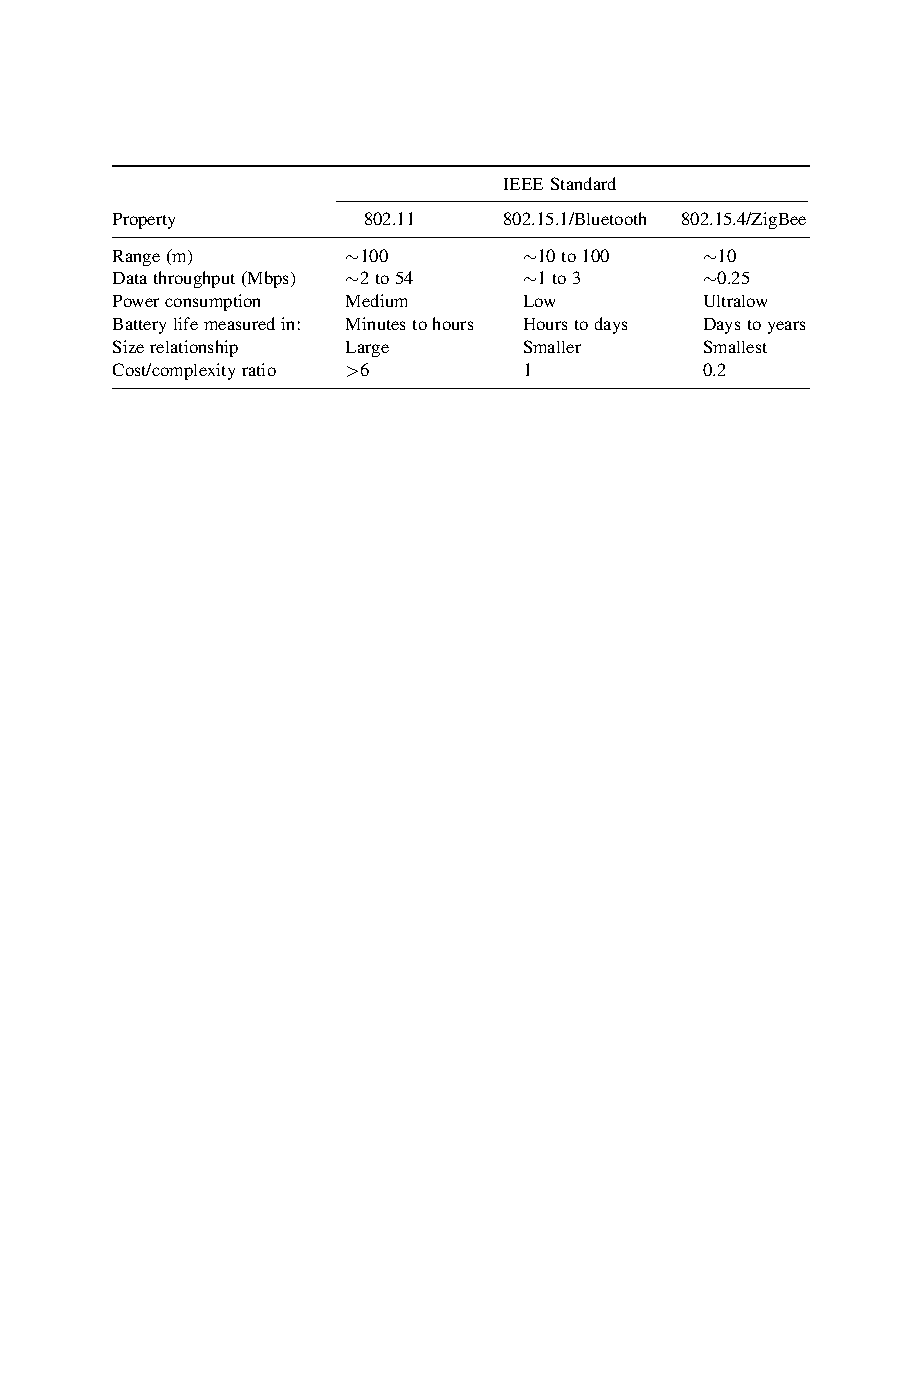
\includegraphics[width=0.8\textwidth]{00images/protocol-comparison}
    \caption{Comparison of IEEE standards for selected physical layer protocols. Taken from~\cite{Sohraby2007WirelessApplications}.}
    \label{fig:protocol-comparison}
\end{figure}
\subsection{MAC layer technologies}

In this section we will explore different \acrshort{mac} technologies that could be used in our system. In figure~\ref{fig:mac-categories} on page \pageref{fig:mac-categories}, some examples of widely-used approaches to the MAC layer are given. However, due to power-consumption constraints of sensors, these may not be suitable in \acrshort{wsn} scenario~\cite{Sohraby2007WirelessApplications}. In the following paragraphs we narrow our considerations to the following three protocols, that have been introduced specifically for WSNs:
\begin{itemize}[noitemsep]
    \item \acrfull{leach}
    \item \acrfull{smacs}
    \item Bluetooth
\end{itemize}

\paragraph{LEACH}
\acrshort{leach} is a protocol that organises sensors randomly into clusters. Each cluster has a dedicated sensor, posing as the \textit{cluster head}. Sensors within a cluster only communicate with the cluster heads, while cluster heads communicate with the sink (more on the architecture of the \acrshort{leach} protocol in the following section.

LEACH uses \acrfull{tdma} to coordinate transmissions within the cluster. During the setup phase, the cluster head receives messages from all the nodes that would like to be part of the cluster. The cluster head then creates a \acrshort{tdma} schedule for all the participating nodes. The nodes switch off their radio, if it is not their time to broadcast or if they have no data to transmit. Since transmitting and listening on the network amount for a significant part of the energy consumption of a node, switching the radio off can increases the power efficiency~\cite{Sohraby2007WirelessApplications, Heinzelman2000Energy-efficientNetworks}.

To prevent interference among different clusters, \acrshort{leach} also uses \acrfull{cdma}. Every cluster uses different set of codes, which are also chosen by the cluster head. This way, every node in the cluster filters incoming messages with the code of its respective cluster and thus does not need to process messages incoming from neighbouring clusters, as these will become filtered out~\cite{Heinzelman2000Energy-efficientNetworks}.

\paragraph{SMACS}
\acrshort{smacs} is a flat-level structure. There are no clusters and cluster heads, instead each node talks with its immediate neighbours. In \acrlong{smacs}, nodes carry out a procedure to discover their neighbours. While \acrshort{tdma} is used throughout the whole network, a \textit{superframe} is maintained by every node to enable the neighbour-discovery process. During this process, the node assigns a time frame to all of its neighbours and every node maintains its own \acrshort{tdma} table, next to the superframe. This way, the node only talks to one of its neighbours at a time. For every such link, a different random \acrshort{cdma} code or \acrshort{fdma} frequency is used to avoid interference among different links that (coincidentally) share the same time slot~\cite{Sohraby2007WirelessApplications, Sohrabi2000ProtocolsNetwork}.

\paragraph{Bluetooth}
Nodes in Bluetooth network form small local clusters called \textit{piconets}. Piconet can include up to seven slave devices and one master device. The master device is responsible for coordinating access of the slave devices to the shared channel and for relaying messages inside and outside of the piconet. Bluetooth is based on \acrshort{tdma} where each slave in piconet has dedicated time slot during which it can transmit. The schedule is decided and maintained by the master device. To save energy, slave devices can enter one of the power-conservation modes~\cite{Haartsen2000TheSystem, Sohraby2007WirelessApplications}:
\begin{itemize}[noitemsep]
    \item \textbf{Sniff mode}, during which the device wakes up regularly, but the sleep time is longer, when compared to active mode.
    \item During the \textbf{hold mode}, device goes to sleep once, but for prolonged amount of time. After this time has elapsed, the devices goes back to active mode.
    \item When in \textbf{park mode}, the device goes to sleep for an indefinite amount of time and needs to be waken up by an external event.
\end{itemize}

\paragraph{Conclusion}
To prevent possible interference among adjacent containers, it would be beneficial to avoid flat-level structure. Both Bluetooth and LEACH form structures where one node is superior to the other nodes. Sink could be this superior node as it is not battery-dependant. Bluetooth only supports eight devices in a piconet, but this should be sufficient for the number of sensors in a reefer container. The ability of \acrshort{leach} to form clusters is an advantage in networks with greater amount of nodes and it may be unnecessarily complex for our scenario.
\subsection{Network layer technologies}
The simplest path discovery algorithm is flooding, where all nodes are peers (flat routing). A sensor node simply broadcast a packet to all of its neighbours, which do the same until a packet reaches the destination. This introduces a problem of the packet circling a network indefinitely, which may be countered by hop count or time to leave field; when the packet is forwarded through a node its hop count is decremented until zero is reached or time to leave is incremented until given number is reached and then it is discarded. Even thought this approach is simple and does not require costly topology or network maintenance it has a drawbacks like traffic implosion (same packet delivered from different nodes to the same one), overlap problem (neighbouring nodes sense similar data info and send them to the same node) or resource blindness (this approach does not care about resource efficiency e.g. power source may be depleted fats).

Gossiping is an approach for path discovery which improve the flooding approach and its shortcomings. In here, the node randomly sends a packet to only one of its neighbours. This way the traffic implosion and overlap problem are overcome. However, it is not suitable for use in extensive networks as this approach explores only one path at the time which would be very time consuming. 

More advanced routing approach is \acrfull{spin}, which is based on negations, as the name already suggest. It faces shortcomings of Flooding and Gossiping namely resource blindness (power source of highly active nodes is depleted quickly), overlapping or performance of network as they grow in size. \acrshort{spin} is data-centric. When a node has a packet to send, there are three steps in the process. First step is an \texttt{ADV} (advertisement) query with metadata sent to all neighbouring nodes, suggesting what data are being send and asking for transmission. Nodes that are willing to receive and re-transmit the data responds with \texttt{REQ} (request) message. Then the node sends \texttt{DATA} (header + metadata + packet) to all nodes that requested those data. So, there are three types of messages in total: \texttt{ADV}, \texttt{REQ} and \texttt{DATA}. The process may be seen in Figure~\ref{fig:spin-protocol}. Data negotiation process happens when the node asks its neighbours (\texttt{ADV}) to send them data and neighbours learns about what data will be send from metadata. Based on the metadata and resource adaptation process (keeps track of power source level and consumption and if the power source level is too low, it will not request the data, which prolongs node’s lifetime) a node decides whether it will request data from the sender or not.

\begin{figure}[ht]
    \centering
    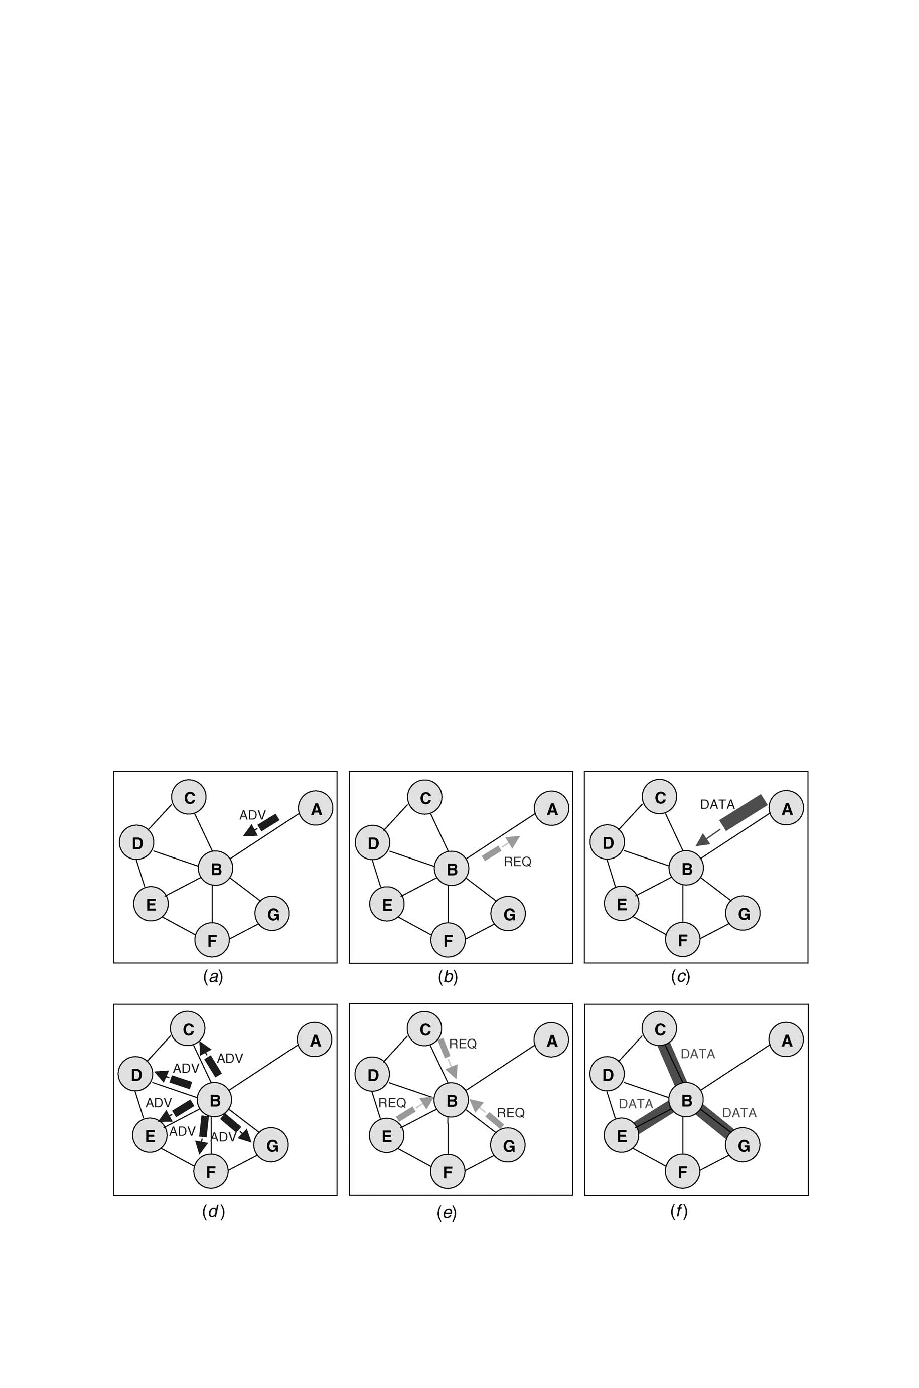
\includegraphics[width=0.8\textwidth]{00images/spin-protocol}
    \caption[itemize]{Operation of the \acrshort{spin} protocol:
    \begin{enumerate*}[label=(\alph*)]
        \item Node A sends ADV query to all its neighbours (B)
        \item Node B receives ADV and decides to accept data, REQ query is send back to node A
        \item Node A sends DATA to node B.
        \item Node B sends ADV query to all its neighbours (C, D, E, F, G)
        \item Nodes C, D, E, F, G receive ADV but only nodes C, E and G decides to accept data and to send REQ query to node A
        \item Node A sends DATA to nodes C, E, G
    \end{enumerate*}
    Figure taken from~\cite{Sohraby2007WirelessApplications}.
    }
    \label{fig:spin-protocol}
\end{figure}

Another approach to routing is \acrfull{leach}, which is based on hierarchical system. Network is divided into clusters with each cluster having a cluster head. The cluster head is responsible of data gathering, its aggregation and transmission to the sink. An assumption is made that each cluster head is one hop from the sink. LEACH has two phases: set-up phase: a cluster head is chosen, and a cluster formed, and steady phase: messages are collected, aggregated and transmitted by a cluster head. This approach achieves significant power saving because of message aggregation and because of master head rotation throughout nodes, all of them are utilised approximately the same. No global information besides who cluster heads are needed as local cluster management is used. Shortcomings of \acrshort{leach} are one-hop assumption from a cluster head to the sink, which is not always true as the cluster head position is rotating and different nodes are at different positions needing more or less power to transmit data to sink when being cluster heads, then choosing a right steady-phase duration is crucial to not deplete one node too much.

\acrfull{pegasus} and hierarchical \acrshort{pegasus} are routing protocols which gather information. They assume that there is a global knowledge of where each node in the network is. \acrshort{pegasus} family uses chain structure. The chain formation is as follows: the furthest node from the sink is selected, then it adjusts its signal strength so that only one neighbour is in reach and makes a connection with it; this way it follows until the sink is reached. For data transmission a chain leader must be chosen (is selected randomly), which is changed every round. Then it gives a token to the rightmost node of the chain from him, which may start sending data down the chain until they reach the chain leader; the same process is then repeated for the leftmost node. When all data are aggregated, the chain leader transmit all data to the sink (it may need to adjust it signal strength to do that) and chain leader is changed. This process is rather slow, and therefore if all nodes are equipped with \acrshort{cdma} transmitter, they may send data to its pair neighbour partner until the chain leader is reached, as it may be seen in Figure~\ref{fig:chain-pegasis}.

\begin{figure}[ht]
    \centering
    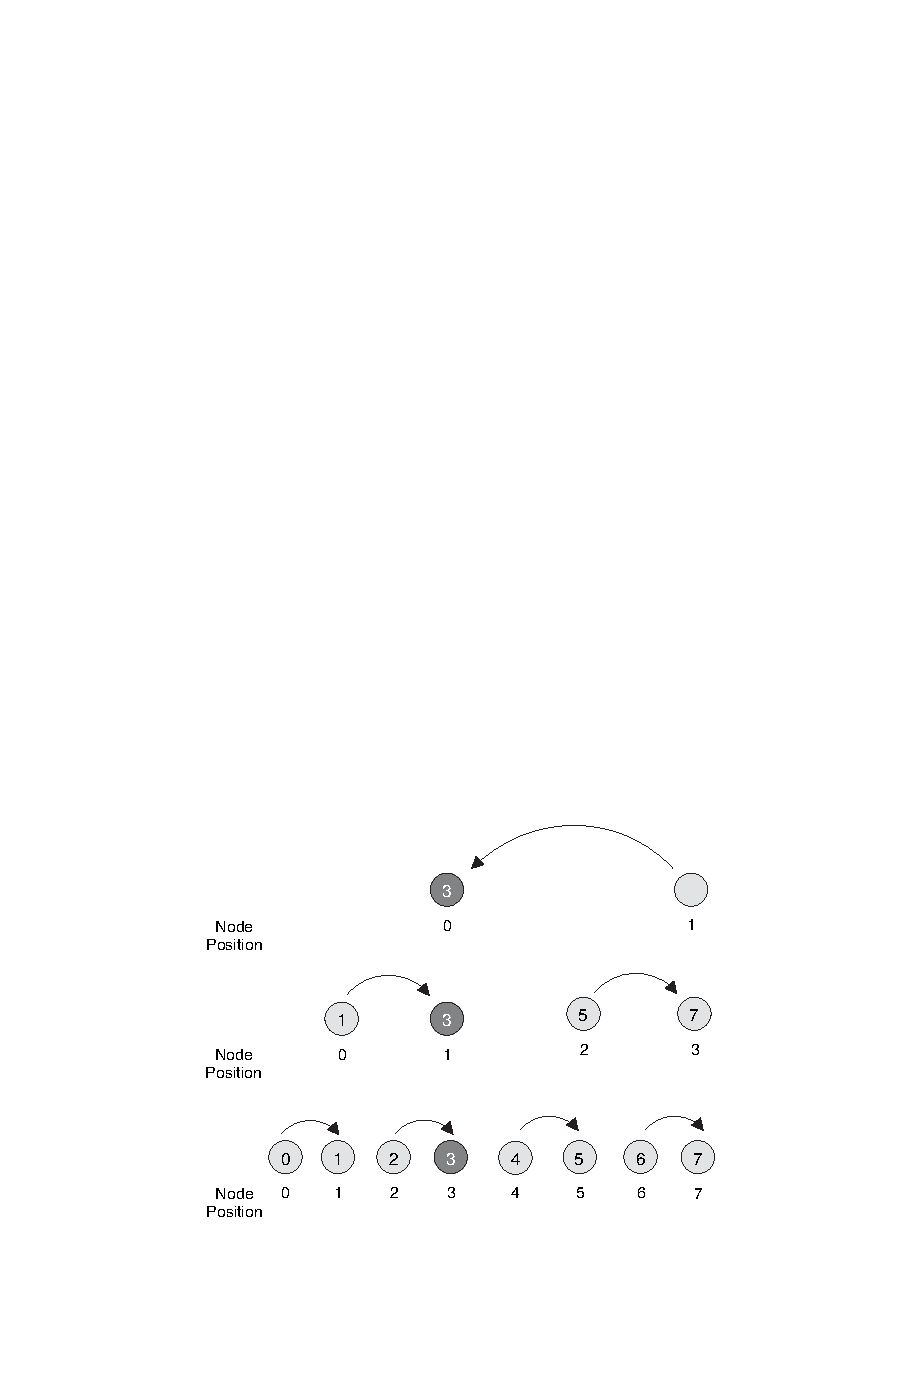
\includegraphics[width=0.8\textwidth]{00images/chain-pegasis}
    \caption{Chain structure of \acrshort{pegasus}. In first step all left nodes in nodes pairs send data to their pair neighbour. This process is repeated and new neighbour pairs are being created as well, until all data are aggregated at the chain leader. Taken from~\cite{Sohraby2007WirelessApplications}}
    \label{fig:chain-pegasis}
\end{figure}

\paragraph{Conclusion}
As may it may have been read at the beginning of this report, our proposed system is made out of two parts: network within a single container and a network on the vessel. Now an analysis of which routing approach or protocol is suitable the most for the given case will be conducted. 
In the case of a network within a container, the most important requirement would be power efficiency. The reason is that sensors within the container are desired to be wireless without cables, neither power cables. Rest of requirements are on the same level, because a delay does not play a big role as long as data are delivered and data to be delivered are not life-threatening, so if it happens that they will not be delivered, nothing happens. There are no more requirements or restrictions than these, so a suggested routing approach is Gossiping. The main reason is the number of sensors within a container which are expected not to be more than to be counted in tens. This suggest rather a smaller wireless sensor network with one sink, where it will not take so long for a packet to be delivered from the sending node to the sink, also it is cheap to produce such sensor.

\acrshort{wsn} on the vessel on the other hand will have more complex structure, and containers within a range of the base station will be constantly changing, and a number of nodes would be counted in thousands. However, power consumption constrains will not be a problem as on the vessel each container will be connected to a power source and so the node’s transmitter. Also, delay and message delivery do not play a big role. The most suitable routing approaches suggested are therefore \acrshort{leach} and \acrshort{pegasus} (with \acrshort{cdma}), as Flooding, Gossiping and \acrshort{spin} are not suitable for networks of this size.


\subsection{Transport layer technologies}
% 
\pagebreak
\printbibliography[heading=bibintoc]
\pagebreak


\end{document}
